\section{Evaluasi}
	Pada subbab ini, penulis akan memaparkan hasil analisa terhadap aplikasi, perspektif non-IT terhadap pengerjaan maupun lingkup pekerjaan dari aplikasi Lelang Online ini.
	
	\subsection{\textit{Summary} Pengujian Fungsionalitas}
	
	\subsection{Pendekatan Hukum Perlindungan Konsumen}
	
	Sebagaimana lelang online adalah salah satu jenis dari jenis transaksi jual-beli barang, tentu saja dalam pelaksanaannya diatur oleh undang-undang dan diawasi pemerintah, terutama untuk lelang harta-harta berharga seperti surat tanah, mobil, ijin usaha, dan lain-lain. Namun, penulis sadar banyak sekali kekurangan pengkajian hukum dan peraturan-peraturan penting seperti hak-hak dan kewajiban masing-masing pihak, \textit{rule} agar lelang dapat berjalan dan diawasi dengan baik, dan peraturan lainnya\\
	Untuk mempermudah pembahasan dan agar pemaparannya lebih kredibel (karena penulis tidak \textit{capable} dan kredibel untuk memaparkan hal ini), maka penulis mengutip sebuah kasus penipuan online - dalam sebuah pertanyaan di platform konsultasi hukum online. Platform online ini - hukumonline.com. Pada platform ini, sering terdapat kajian kasus-kasus hukum dan menggunakan pendekatan hukum untuk penyelesaiannya. Dalam kasus ini, setelah berdiskusi dengan teman dan saudara yang mengambil spesialisasi hukum, penulis dengan hati-hati memaparkan sesuai dengan poin-poin yang persis ada dalam forum online tersebut, dan tidak mengubah satupun kata agar kebenaran informasi yang disampaikan tidak berubah.\\
	\indent Pada keterangannya, pengkajian kasus ini menggunakan pendekatan utama pada \textbf{Undang-Undang Nomor 8 Tahun 1999 tentang Perlindungan Konsumen ("UU PK") } dan \textbf{Peraturan Pemerintah Nomor 82 Tahun 2012 tentang Penyelenggaraan Sistem dan Transaksi Elektronik ("PP PSTE") }. PP PSTE sendiri merupakan turunan dari \textbf{Undang-Undang Nomor 11 Tahun 2008 tentang Informasi dan Transaksi Elekronik ("UU ITE")}.
	\subsubsection{Perlindungan Hukum Bagi Konsumen Belanja \textit{Online}}
	Pemaparan subbab ini berupa pertanyaan yang dikaji dalam hukumonline.com, disajikan dalam bentuk pertanyaan dan jawaban.\\
\textbf{Pertanyaan}
\begin{displayquote}
	Saya pernah belanja barang secara online, tapi barang yang saya beli tidak sama dengan yang saya lihat di foto pada iklan yang dipajang. Pertanyaan saya, apakah itu termasuk pelanggaran hak konsumen? Apakah saya dapat menuntut penjual untuk mengembalikan uang atau mengganti barang yang saya beli tersebut? Terima kasih.
\end{displayquote}


\textbf{Jawaban oleh hukumonline.com: \\ Pendekatan Hukum Perlindungan Konsumen dalam Transaksi Jual Beli/Belanja secara \textit{Online}} \\ \ \\
\indent Dengan pendekatan UU Perlindungan Konsumen, kasus yang Anda sampaikan tersebut dapat kami simpulkan sebagai salah satu pelanggaran terhadap hak konsumen. \\

\indent Pasal 4 UU PK menyebutkan bahwa hak konsumen/dalam kasus ini adalah pengguna aplikasi lelang online adalah sebagai berikut:
\begin{enumerate}[label=\alph*.]
	\item hak atas kenyamanan, keamanan, dan keselamatan dalam mengkonsumsi barang dan/atau jasa;
	\item hak untuk memilih barang dan/atau jasa serta mendapatkan barang dan/atau jasa tersebut sesuai dengan nilai tukar dan kondisi serta jaminan yang dijanjikan;
	\item \textbf{hak atas informasi yang benar, jelas, dan jujur mengenai kondisi dan jaminan barang dan/atau jasa};
	\item hak untuk didengar pendapat dan keluhannya atas barang dan/atau jasa yang digunakan;
	\item \textbf{hak untuk mendapatkan advokasi, perlindungan, dan upaya penyelesaian sengketa perlindungan konsumen secara patut};
	\item hak untuk mendapat pembinaan dan pendidikan konsumen;
	\item hak unduk diperlakukan atau dilayani secara benar dan jujur serta tidak diskriminatif;
	\item \textbf{hak untuk mendapatkan kompensasi, ganti rugi dan/atau penggantian, apabila barang dan/atau jasa yang diterima tidak sesuai dengan perjanjian atau tidak sebagaimana mestinya};
	\item hak-hak yang diatur dalam ketentuan peraturan perundangundangan lainnya.
\end{enumerate}

\indent Di sisi lain, kewajiban bagi pelaku usaha (dalam hal ini adalah penjual online), sesuai Pasal 7 UU PK adalah:
\begin{enumerate}[label=\alph*.]
	\item beritikad baik dalam melakukan kegiatan usahanya;
	\item \textbf{memberikan informasi yang benar, jelas dan jujur mengenai kondisi dan jaminan barang dan/atau jasa serta memberi penjelasan penggunaan, perbaikan dan pemeliharaan};
	\item memperlakukan atau melayani konsumen secara benar dan jujur serta tidak diskriminatif;
	\item \textbf{menjamin mutu barang dan/atau jasa yang diproduksi dan/atau diperdagangkan berdasarkan ketentuan standar mutu barang dan/atau jasa yang berlaku};
	\item \textbf{memberi kesempatan kepada konsumen untuk menguji, dan/atau mencoba barang  dan/atau jasa tertentu serta memberi jaminan dan/atau garansi atas barang yang dibuat dan/atau yang diperdagangkan};
	\item \textbf{memberi kompensasi, ganti rugi dan/atau penggantian atas kerugian akibat penggunaan, pemakaian dan pemanfaatan barang dan/atau jasa yang diperdagangkan};
	\item \textbf{memberi kompensasi, ganti rugi dan/atau penggantian apabila barang dan/atau jasa yang diterima atau dimanfaatkan tidak sesuai dengan perjanjian}.
\end{enumerate}\ \\

\indent Selaku konsumen sesuai Pasal 4 huruf h UU PK tersebut, berhak mendapatkan kompensasi, ganti rugi dan/atau penggantian apabila barang dan/atau jasa yang diterima tidak sesuai dengan perjanjian atau tidak sebagaimana mestinya. Sedangkan, pelaku usaha itu sendiri sesuai Pasal 7 huruf (g) UU PK berkewajiban memberi kompensasi, ganti rugi dan/atau penggantian apabila barang dan/atau jasa yang diterima atau dimanfaatkan tidak sesuai dengan perjanjian.\\

\indent Apabila pelaku usaha (dalam hal ini, penulis karena penulis sebagai perantara antara pelelang dan pembeli) tidak melaksanakan kewajibannya, pelaku usaha dapat dipidana berdasarkan Pasal 62 UUPK, yang berbunyi:
\begin{displayquote}
	"Pelaku usaha yang melanggar ketentuan sebagaimana dimaksud dalam Pasal 8, Pasal 9, Pasal 10, Pasal 13 ayat (2), Pasal 15, Pasal 17 ayat (1) huruf a, huruf b, huruf c, huruf e, ayat (2) dan Pasal 18 dipidana dengan \textbf{pidana penjara paling lama 5 (lima) tahun} atau pidana denda paling banyak \textbf{Rp 2.000.000.000,00 (dua milyar rupiah)}".
\end{displayquote}

\subsubsection{Kontrak Elektronik dan Perlindungan Konsumen berdasarkan UU ITE dan PP PSTE}
Transaksi jual beli Anda, meskipun dilakukan secara online, berdasarkan UU ITE dan PP PSTE tetap diakui sebagai transaksi elektronik yang dapat dipertanggungjawabkan. Persetujuan konsumen untuk membeli barang secara \textit{online} dengan cara melakukan klik persetujuan atas transaksi merupakan bentuk tindakan penerimaan yang menyatakan persetujuan dalam kesepakatan pada transaksi elektronik. Tindakan penerimaan tersebut biasanya didahului pernyataan persetujuan atas syarat dan ketentuan jual beli secara online yang dapat kami katakan juga sebagai salah satu bentuk \textbf{Kontrak Elektronik}. Kontrak Elektronik menurut \textbf{Pasal 47 ayat (2) PP PSTE} dianggap sah apabila:
\begin{enumerate}[label=\alph*.]
	\item terdapat kesepakatan para pihak;
	dilakukan oleh subjek hukum yang cakap atau yang berwenang mewakili sesuai dengan ketentuan peraturan \item perundang-undangan;
	\item terdapat hal tertentu; dan
	\item objek transaksi tidak boleh bertentangan dengan peraturan perundang-undangan, kesusilaan, dan ketertiban umum.
\end{enumerate}
\ \\
\indent Kontrak Elektronik itu sendiri menurut \textbf{Pasal 48 ayat (3) PP PSTE} setidaknya harus memuat hal-hal sebagai berikut:
\begin{enumerate}[label=\alph*.]
	\item data identitas para pihak;
	\item objek dan spesifikasi;
	\item persyaratan Transaksi Elektronik;
	\item harga dan biaya;
	\item prosedur dalam hal terdapat pembatalan oleh para pihak;
	\item ketentuan yang memberikan hak kepada pihak yang dirugikan untuk dapat mengembalikan barang dan/atau meminta penggantian produk jika terdapat cacat tersembunyi; dan
	\item pilihan hukum penyelesaian Transaksi Elektronik.
\end{enumerate}
\ \\
\indent Terkait dengan perlindungan konsumen, \textbf{Pasal 49 ayat (1) PP PSTE menegaskan bahwa Pelaku Usaha yang menawarkan produk melalui Sistem Elektronik wajib menyediakan informasi yang lengkap dan benar berkaitan dengan syarat kontrak, produsen, dan produk yang ditawarkan.}

\subsubsection{\textit{Summary}}
	\indent Untuk mencapai hasil pengujian yang maksimal, seharusnya aplikasi lelang online ini melakukan tes pasar/tes pengguna, dimana aplikasi ini benar-benar \textit{dilempar} ke pasar, lewat iklan/\textit{endorsements}/\textit{digital advertising} lainnya. Penulis sudah mempersiapkan aplikasi untuk dapat melakukan tes pasar, yaitu \textit{hosting} aplikasi, pembelian domain sedemikian rupa agar aplikasi ini dapat diakses masyarakat luas dan benar-benar siap untuk tes pasar.\\
	\indent Sebenarnya penulis sudah merencanakan cara-cara untuk pemasaran agar tes pengguna ini berlangsung dengan baik, namun penulis sadar bahwa dalam proses pengerjaan maupun saat \textit{requirement gathering}, sangat sedikit pertimbangan hukum (seperti peraturan lelang yang adil, proses pengawasan lelang yang sesuai dengan peraturan pemerintah, dll) dimasukkan dalam proses pembuatan aplikasi, sementara proses jual-beli itu sendiri proses yang vital dan hak kewajiban masing-masing pelaku (baik pembeli, penjual dan ) diatur dalam undang-undang. \\ 
	\indent Poin-poin yang dicetak tebal pada pemaparan pasal 4 dan pasal 7 UU PK adalah poin-poin yang tidak bisa penulis penuhi sebagai pelaku usaha dalam pengerjaan tugas akhir ini. Terkait dengan sanksi dan pidana yang menunggu jika penulis tetap menjalankan tes pasar tanpa mengikuti undang-undang yang ada, inkapabilitas penulis dalam sebagai penyelenggara usaha (lelang online), maka penulis memutuskan untuk tidak melakukan tes pasar.
	\\

	Dasar hukum yang digunakan (tetap dikutip dari hukumonline.org):
	\begin{enumerate}
		\item Kitab Undang-Undang Hukum Pidana
		\item Undang-Undang Nomor 8 Tahun 1999 tentang Perlindungan Konsumen
		\item Undang-Undang Nomor 11 Tahun 2008 tentang Informasi dan Transaksi Elekronik
		\item Peraturan Pemerintah Nomor 82 Tahun 2012 tentang Penyelenggaraan Sistem dan Transaksi Elektronik
	\end{enumerate}
			
	\subsection{\textit{Summary} Pengujian Pengguna}
	\indent Rekapitulasi tersebut diurutkan berdasarkan besarnya/signifikansi persentase perbedaan antara kedua platform, dapat dilihat pada Tabel \ref{user-test-recap-sorted}.
\LTXtable{\textwidth}{table/05/pengguna/recap_sorted}

Visualisasi perbandingan dapat dilihat lewat diagram garis pada Gambar \ref{diagram-pengguna-chart}.

\begin{figure}[H]
	\centering
	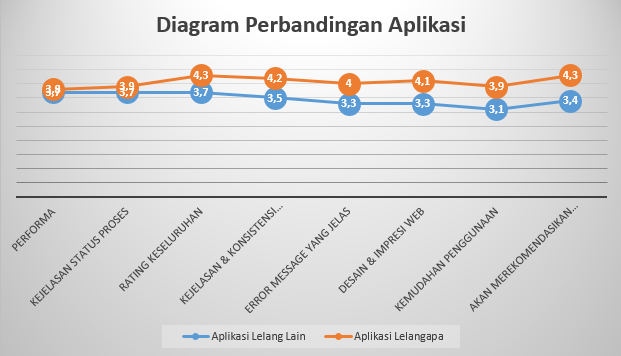
\includegraphics[width=\textwidth]{images/bab5/ujipengguna/chart.png}
	\caption{Diagram perbandingan pengujian \textit{user experience} pengguna}
	\label{diagram-pengguna-chart}
\end{figure}

Dalam hal ini, dapat disimpulkan bahwa impresi \textit{user experience} sudah baik, dan skor \textit{user experience}nya sedikit diatas sistem serupa lainnya. Perbedaannya sudah cukup signifikan adalah \textit{recommendation}, kemudahan penggunaan dan desain web yang baik. Namun, yang menjadi perhatian adalah perbedaan \textit{performa} yang masih sangat kecil. Hal ini terkait dengan pengujian \textit{speed test} di subbab selanjutnya.
	
	\subsection{\textit{Further Enchancements}}
	

	